\documentclass{standalone}
  \usepackage{tikz}
  \usetikzlibrary{arrows.meta, automata, bending, positioning, shapes.misc}
  \tikzstyle{automaton}=[shorten >=1pt, >={Stealth[bend,round]}, initial text=]
  \tikzstyle{accepting}=[double]

\begin{document}
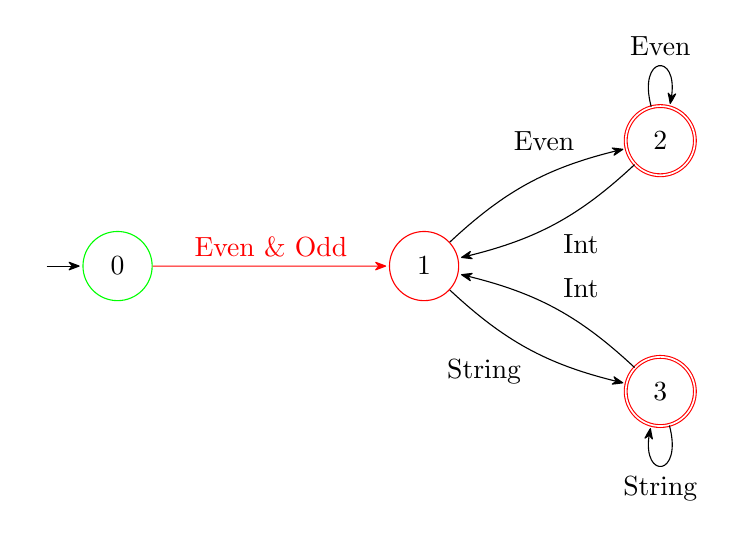
\begin{tikzpicture}[automaton, auto]
  \node[state,color=green,text=black,initial,rounded rectangle] (0) {$0$};
  \node[state,color=red,text=black,rounded rectangle] (1) [right=30mm of 0] {$1$};
  \node[state,color=red,text=black,accepting,rounded rectangle] (2) [above right=7mm and 30mm of 1] {$2$};
  \node[state,color=red,text=black,accepting,rounded rectangle] (3) [below right=7mm and 30mm of 1] {$3$};
  \path[->] (0) edge[color=red] node {Even \& Odd} (1);
  \path[->] (1) edge[bend left=15]  node[pos=.8] {Even} (2);
  \path[->] (1) edge[bend right=15] node[swap] {String} (3);
  \path[->] (2) edge[bend left=15]  node {Int} (1);
  \path[->] (2) edge[loop above]    node {Even} (2);
  \path[->] (3) edge[bend right=15] node[swap] {Int} (1);
  \path[->] (3) edge[loop below]    node {String} (3);
\end{tikzpicture}
\end{document}
